\documentclass[11pt,a4paper]{report}%especifica o tipo de documento que tenciona escrever: carta, artigo, relatório... neste caso é um relatório
% [11pt,a4paper] Define o tamanho principal das letras do documento. caso não especifique uma delas, é assumido 10pt
% a4paper -- Define o tamanho do papel.
\usepackage{float}
\usepackage[portuges]{babel}%Babel -- irá activar automaticamente as regras apropriadas de hifenização para a língua todo o
                                   %-- o texto gerado é automaticamente traduzido para Português.
                                   %  Por exemplo, “chapter” irá passar a “capítulo”, “table of contents” a “conteúdo”.
                                   % portuges -- específica para o Português.
\usepackage[utf8]{inputenc} % define o encoding usado texto fonte (input)--usual "utf8" ou "latin1

\usepackage{graphicx} %permite incluir graficos, tabelas, figuras
\usepackage{url} % para utilizar o comando \url{}
\usepackage{enumerate} %permite escolher, nas listas enumeradas, se os iems sao marcados com letras ou numeros-romanos em vez de numeracao normal

%\usepackage{apalike} % gerar biliografia no estilo 'named' (apalike)

\usepackage{color} % Para escrever em cores

\usepackage{multirow} %tabelas com multilinhas
\usepackage{array} %formatação especial de tabelas em array

\usepackage[pdftex]{hyperref} % transformar as referências internas do seu documento em hiper-ligações.

%Exemplos de fontes -- nao e vulgar mudar o tipo de fonte
%\usepackage{tgbonum} % Fonte de letra: TEX Gyre Bonum
%\usepackage{lmodern} % Fonte de letra: Latin Modern Sans Serif
%\usepackage{helvet}  % Fonte de letra: Helvetica
%\usepackage{charter} % Fonte de letra:Charter

\definecolor{saddlebrown}{rgb}{0.55, 0.27, 0.07} % para definir uma nova cor, neste caso 'saddlebrown'

\usepackage{listings}  % para utilizar blocos de texto verbatim no estilo 'listings'
%paramerização mais vulgar dos blocos LISTING - GENERAL
\lstset{
	basicstyle=\small, %o tamanho das fontes que são usadas para o código
	numbers=left, % onde colocar a numeração da linha
	numberstyle=\tiny, %o tamanho das fontes que são usadas para a numeração da linha
	numbersep=5pt, %distancia entre a numeração da linha e o codigo
	breaklines=true, %define quebra automática de linha
    frame=tB,  % caixa a volta do codigo
	mathescape=true, %habilita o modo matemático
	escapeinside={(*@}{@*)} % se escrever isto  aceita tudo o que esta dentro das marcas e nao altera
}
%
%\lstset{ %
%	language=Java,							% choose the language of the code
%	basicstyle=\ttfamily\footnotesize,		% the size of the fonts that are used for the code
%	keywordstyle=\bfseries,					% set the keyword style
%	%numbers=left,							% where to put the line-numbers
%	numberstyle=\scriptsize,				% the size of the fonts that are used for the line-numbers
%	stepnumber=2,							% the step between two line-numbers. If it's 1 each line
%											% will be numbered
%	numbersep=5pt,							% how far the line-numbers are from the code
%	backgroundcolor=\color{white},			% choose the background color. You must add \usepackage{color}
%	showspaces=false,						% show spaces adding particular underscores
%	showstringspaces=false,					% underline spaces within strings
%	showtabs=false,							% show tabs within strings adding particular underscores
%	frame=none,								% adds a frame around the code
%	%abovecaptionskip=-.8em,
%	%belowcaptionskip=.7em,
%	tabsize=2,								% sets default tabsize to 2 spaces
%	captionpos=b,							% sets the caption-position to bottom
%	breaklines=true,						% sets automatic line breaking
%	breakatwhitespace=false,				% sets if automatic breaks should only happen at whitespace
%	title=\lstname,							% show the filename of files included with \lstinputlisting;
%											% also try caption instead of title
%	escapeinside={\%*}{*)},					% if you want to add a comment within your code
%	morekeywords={*,...}					% if you want to add more keywords to the set
%}

\usepackage{xspace} % deteta se a seguir a palavra tem uma palavra ou um sinal de pontuaçao se tiver uma palavra da espaço, se for um sinal de pontuaçao nao da espaço

\parindent=0pt %espaço a deixar para fazer a  indentação da primeira linha após um parágrafo
\parskip=2pt % espaço entre o parágrafo e o texto anterior

\setlength{\oddsidemargin}{-1cm} %espaço entre o texto e a margem
\setlength{\textwidth}{18cm} %Comprimento do texto na pagina
\setlength{\headsep}{-1cm} %espaço entre o texto e o cabeçalho
\setlength{\textheight}{23cm} %altura do texto na pagina

% comando '\def' usado para definir abreviatura (macros)
% o primeiro argumento é o nome do novo comando e o segundo entre chavetas é o texto original, ou sequência de controle, para que expande
\def\darius{\textsf{Darius}\xspace}
\def\antlr{\texttt{AnTLR}\xspace}
\def\pe{\emph{Publicação Eletrónica}\xspace}
\def\titulo#1{\section{#1}}    %no corpo do documento usa-se na forma '\titulo{MEU TITULO}'
\def\super#1{{\em Supervisor: #1}\\ }
\def\area#1{{\em \'{A}rea: #1}\\[0.2cm]}
\def\resumo{\underline{Resumo}:\\ }

%\input{LPgeneralDefintions} %permite ler de um ficheiro de texto externo mais definições

\title{Processamento de Linguagens (3º ano de Curso)\\
       \textbf{Trabalho Prático 1}\\ Relatório de Desenvolvimento
       } %Titulo do documento
%\title{Um Exemplo de Artigo em \LaTeX}
\author{José Pereira\\ (a82880@alunos.uminho.pt) \and Ricardo Petronilho\\ (a81744@alunos.uminho.pt)
       } %autores do documento
\date{\today} %data

\begin{document} % corpo do documento
\maketitle % apresentar titulo, autor e data

\begin{abstract}  % resumo do documento
O projeto elaborado na Unidade Curricular de Processamento de Linguagens do Mestrado integrado em Engenharia Informática da Universidade do Minho, tem como principal objetivo o processamento de informação contida em ficheiros que incluem citações de autores, através de expressões regulares utilizando a ferramenta flex.
\end{abstract}

\tableofcontents % Insere a tabela de indice
%\listoffigures % Insere a tabela de indice figuras
%\listoftables % Insere a tabela de indice tabelas

\chapter{Introdução} \label{chap:intro} %referência cruzada

Na unidade curricular de Processamento de Linguagens, do Mestrado integrado em Engenharia Informática da Universidade do Minho, foi nos proposta a elaboração do exerício 6, que se trata da elaboração de um programa que através da ferramenta flex, processa ficheiros, sendo o principal objetivo filtrar as informações mais importantes.\\\\
Deste modo, os ficheiros analisados contém citações de autores e as respetivas traduções, sendo que, algumas das citações tem autor desconhecido.\\\\Para a elaboração deste programa, foi necessária uma análise rigorosa do ficheiro que contém as citações, para encontrar as expressões regulares para cada tipo de informação. \\\\Por fim, em trabalho adicional elaborou-se a geração de uma página HTML, com os autores e as respetivas citações/traduções. Do mesmo modo, também se elaborou uma estatística e geração de uma mensagem aleatório do dia.


\chapter{Análise e Especificação} \label{chap:analiseEspecificacao} %capitulo e referencia cruzada
\section{Contextualização do problema} \label{sec:descricaoProblema} %seccao e referencia cruzada
O objetivo central deste trabalho prático é focado no processamento da informação de grandes ficheiros.\\\\Neste caso, tal como já foi referenciado anteriormente o ficheiro para processamento contém citações e traduções das mesmas, que podem estar ou não associadas a autores.\\\\Deste modo, utilizando a ferramenta flex, que gera programas que realizam correspondência de padrões em texto, espera-se filtrar páginas, que podem ou não estar associadas a um autor e as suas respetivas citações, e traduções, as quais contém diferentes padrões de identificação.


\chapter{Concepção/desenho da Resolução}

\section{Padrões detetados}
Com uma análise rigorosa ao ficheiro disponibilizado pela equipa Docente denominado por \emph{ptwikiquote-20190301-pages-articles.xml} foram detetados os seguintes padrões:\\\\

\begin{figure}[ht]
	\centering
	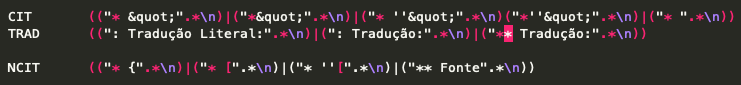
\includegraphics[scale=0.6]{er.png}
	\caption{Padrões detetados.}
	\label{img:cit}
\end{figure}


O \emph{CIT} corresponde às cinco expressões regulares para encontrar citações, começando todas pelo caracter *, o padrão \&quout;, representa as aspas, pelo que depois será normalizado para tal. Por fim existe o caso particular em que pode não existir aspas. \\De seguida, tem-se o \emph{TRAD}, que contém três expressões regulares para encontrar traduções. 
\\Por fim, e não menos importante, foi necesário incluir o \emph{NCIT}, que contém as expressões regulares para não citações. A inclusão deste é necessária pois, como existem expressões que não são citações que começam por *, haveria conflitos com a quinta expressão regular para citações, logo é importante garantir que quando esta ocorre, não é feito qualquer processamento da expressão.


\newpage

\section{Autómato desenhado}

\begin{figure}[H]
	\centering
	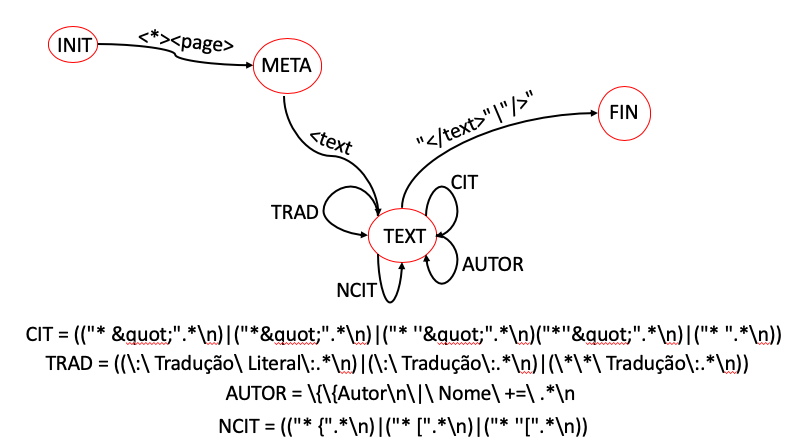
\includegraphics[scale=0.6]{automato.png}
	\caption{Autómato desenhado para o problema.}
	\label{img:automato}
\end{figure}

A figura acima representa o autómato utilizado para a elaboração do programa \emph{parse}. O autómato foi desenvolvido à priori à elaboração do código, o qual facilitou a tomada de decisões que foram imediatamente tomadas no papel, tornando clara de seguida a elaboração do código.\\
Assim, existem quatro possíveis estados, \emph{INIT},\emph{META},\emph{TEXT},\emph{FIN}. O INIT é o estado inicial, ou seja, antes de se processar qualquer expressão, quando se deteta a expressão regular de uma página, passa-se para o estado \emph{META}. O \emph{META} é o estado referente ao header de uma página, sendo que a \emph{TAG} que nos interessa é o text, (como se pode observar na figura 3.3 com a seta laranja), pois é nesta que se encontra toda a informação que pertende-se filtrar, como autores, citações e traduções. Quando é encontrado a \emph{TAG} \emph{text}, passa-se para o estado TEXT, sendo que neste estado podem acontecer cinco situações diferentes.\\\\ 

\begin{figure}[H]
	\centering
	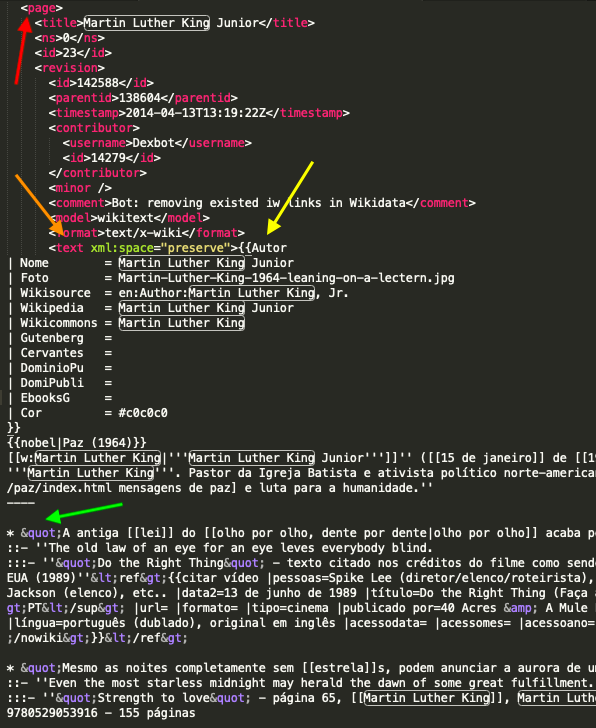
\includegraphics[scale=0.6]{pagina.png}
	\caption{Expressões regulares encontradas no ficheiro.}
	\label{img:pag}
\end{figure}

A primeira situação é ocorrer match com a expressão de \emph{AUTOR} (onde podemos ver especificamente a expressão regular na imagem 3.2 e na figura 3.3 com a seta amarela), o que signifca que se encontrou o nome do mesmo, caso isto ocorra, recolhe-se a informação e volta-se ao estado \emph{TEXT} para se continuar a processar o conteúdo desta página. \\A expressão \emph{CIT}, significa que se encontrou uma citação, pelo que se recolhe a mesma, faz-se a normalização das aspas e volta-se ao estado \emph{TEXT}, (exemplo disto, pode-se observar na figura 3.3 com a seta verde). \\O \emph{NCIT}, é usado para não ocorrer conflitos com as reais citações, tal como já foi referenciado anteriormente, pelo que a ação desta condição não irá fazer nada, apenas garantir que não sejam consideradas citações, voltando apenas para o estado \emph{TEXT}. \\A condição \emph{TRAD} (onde a expressão regular se pode verificar na figura 3.2), representa as traduções, pelo que a ação da mesma, é normalizar as aspas, caso ocorram e imprimir/guardar na estrutura de dados, e voltar ao estado \emph{TEXT}.\\ Por fim, quando é encontrado a expressão do fim da \emph{TAG} text, passa-se para o estado \emph{FIN}, que irá finalizar esta página e passar para a próxima.

\newpage

\section{Algoritmos}

\subsection{Normalização das aspas}
Para a \textbf{normalização das aspas} foi implementado um algoritmo genérico que detando a palavra - \textbf{&quot;} - substitui a mesma pelo caracter - \textbf{''} - obtendo assim o formato das aspas usual. Em suma o algorimto deteta o índice da ocurrência da expressçao - &quot; - e copia a primeira metade da string antes da expressão para a nova string, escreve o caracter - \textbf{''} - e de seguinda copia a segunda metade da string depois da expressão para nova string, obtendo assim, em tempo linear, a string normalizada. A função que implementa este algoritmo tem o seguinte protótipo:\\\\
\textbf{char* normalizaAspas(char* str);}\\\\
O funcionamneto desta função é ilustrado de seguida:\\
A título exemplificativo é passado como parâmetro a string - \textbf{''&quot;ola&quot;''} - a função aloca uma nova string com memória suficiente para armazenar a sub-string - \textbf{''ola&quot;} - já com o caracter das aspas normalizado, removendo assim o primeiro - \textbf{&quot;} - de seguinda deteta a próxima ocurrência da mesma expressão alocando novamente memória para a nova string sem a expressão, no fim é retornado a string normalizada \textbf{''ola''}.\\
Esta função funciona para a normalização de N - \textbf{&quot;} - sendo por isso genérica, desta forma mesmo que a citação ou tradução em causa tenha por exemplo 6 - \textbf{&quot;} - ao longo da sua extensão, a função normaliza todas as ocurências, até caso tenham um número impar de expressões.

\subsection{Hash table com citações de cada autor}

De forma a armazenar as citações organizadamente para cada autor foi utilizada uma \textbf{Hash Table} em que a chave é o nome do autor e o valor correspondente é um \textbf{ArrayList} com todas as citações desse mesmo autor.\\
Foi utilizada a API pública \textbf{GLib} para o manuseamento das estruturas referidas.
Esta estrutura é fundamental para a funcionalidade de indicar uma \textbf{mensagem do dia}. Para tal foram utilizadas aa funções \textbf{srand()} e \textbf{rand()}, gerando uma seed e um número pseudo-aleatório respetivamente no intervalo: 0 - número de autores. Desta forma acedemos a posição N, aleatória, da Hash Table obetendo a lisa de citações do autor, da igual modo, é gerado um novo número aleatório no intervalo: 0 - número de citações do autor, para obter uma citção totalmente aleatória.\\\\
\textbf{Observação:} Para esta funcionalidade em específico chegava ter uma única lista de citações para todos os autores em vez de uma Hash Table, no entanto esta estrutura foi utilizada a pensar no futuro desenvolvimento deste projeto, uma vez que armazenar as citaçoes por autor permite concretizar um maior número de possíveis funcionalidades.


\subsection{Geração de páginas HTML}
Como trabalho adicional a equipa decidiu gerar uma página HTML com a informação dos autores, onde se lista os mesmos que estão presentes no ficheiro .xml, e através de um link tem-se uma página com as citações e traduções do mesmo, sendo importante referir que o grupo, exclui desta funcionalidade as citações sem autor, ou autor sem nome, devido às razões evidênciadas anteriormente. Os ficheiros criados para cadad página de autor, foram nomeados com o respetivo nome do mesmo e colocados numa diretoria chamada \emph{paginas} A esta página html também foi adicionado dados estatísticos acerca do ficheiro como, número de páginas, número de citações, número de autores, número de traduções. Por fim, adicinou-se uma mensagem do dia, onde se escolhe aleatóriamente uma das citações.\\\\
Apesar do programa guardar a informação das citações, autores, etc., numa \emph{HASHTABEL}, os ficheiros .html são gerados ao mesmo tempo que é feito o processamento do ficheiro.xml, pois é mais eficiente, e não trazia qualquer vantagem em fazê-lo depois com a estrutura. \\Como o programa tem a funcionalidade de escrever em ficheiros .txt e gerar páginas HTML, decidiu-se usar um variável global \emph{opcao}, para distinguir os dois processos.


\chapter{Codificação e Testes}
\section{Problemas de Implementação}
Alguns dos problemas que surgiram durante a elaboração do projeto, encontrou-se na dificuldade de identificar todas as expressões regulares para citações e traduções, pois torna-se complicado, devido à diversidade. Deste modo, a equipa tentou-te capturar o maior número de expressões para cada tipo de informação.\\

No momento de codificação da geração de páginas .html o grupo deparou-se com o problema de o próprio nome do autor não ser compatível para possível nome do ficheiro, uma vez que continha caracteres especiais, incompatíveis ou mesmo o próprio nome era vazio. De forma a resolver o problema simplesmente ignorou-se as citações dos mesmos não sendo gerado o respetivo ficheiro .html.\\
Note-se que no entanto estas citações quando executado a versão normal - \textbf{-n} - isto é, quando escritas no ficheiro output.txt são todas apresentadas, mesmo as que não têm autor.

\section{Testes realizados e Resultados}
A forma como o grupo testou o programa foi em primeira instância com pequenos exemplos, com padrões específicos, para deteção de erros, com as expressões regulares. Por fim testou-se exaustivamente com o ficheiro fornecido pela equipa Docente, garantido que eram cumpridos os requesítos sem qualquer falha.


\section{Como Instalar o executável}

Para simplificar a compilação e instalação do executável foi criado um ficheiro -  \textbf{Makefile} - que contém os seguintes comandos:\\

\textbf{make parse\\
make install\\
make uninstall\\
make clean\\}

Para instalar basta evocar - \textbf{make install} - que previamente compila o executável e de seguida copia o mesmo para a diretoria - \textbf{/usr/local/bin/} -
que por pré-definição faz parte da variável de ambiente - \textbf{PATH} - dos sistemas UNIX, desta forma torna-se um programa de sistema.

\section{Como utilizar o executável}

Existem 3 versões de utilização do executável evidenciadas de seguida:\\
 
\textbf{./parse help\\
./parse -n file.xml\\
./parse -m file.xml\\
./parse -h file.xml\\}

Quando digitado - \textbf{help} - é escrito no terminal o tutorial de como utilizar o executável.\\

A opção - \textbf{-n} - significa \textbf{normal} e escreve no ficheiro \textbf{output.txt} todas as citações e respetivas traduções detetadas.\\

A opção - \textbf{-m} - significa \textbf{mensagem do dia} e realiza o que a opção normal faz com o extra de escrever uma citação aleatória num ficheiro á parte denominadado \textbf{message\_of\_the\_day.txt}.\\

A opção - \textbf{-h} - significa \textbf{HTML} e escreve todas citações de autores conhecidos no respetivo ficheiro \textbf{.html} dedicado a cada autor, é gerado também o \textbf{index.html} que contém o link para a página de cada autor.

%\VerbatimInput{teste1.txt}

\chapter{Conclusão}
Em suma, os objetivos inicialmente propostos foram cumpridos, dos quais, a listagem de citações identificadas pelo autor, caso seja conhecido, e as respetivas traduções das citações.\\\\
A análise exaustiva do ficheiro para encontrar os padrões para cada tipo de informação foi importante para atingir o resultado final.\\\\
A primeira etapa realizada pela equipa foi o desenho e análise do autómato, a qual foi imprecindível para a elaboração do projeto, pois tornou mais clara a conceção do código do programa \emph{parse}, sendo que grande parte das decisões ficaram tomadas no papel.\\\\
Não foi possível capturar todo o tipo de citações ou traduções, pois torna-se complicado avaliar todos os padrões presentes no ficheiro.\\\\
Em medida de trabalho adicional ao pedido pela equipa docente, foram elaboradas estatísticas, que na opinião dos membros da mesma são dados importantes após o processamento dos ficheiros. Também foi elaborada a funcionalidade da criação de uma página HTML, onde se listam os autores, com links para páginas onde se encontram as respetivas citações, também ainda na mesma página, encontram-se estatísticas e uma mensagem do dia que é escolhida aleatóriamente.
Assim, conclui-se que o resultado final do projeto de Processamento de Linguagens é o esperado pelo grupo, pelo que existe diversas ideias para trabalho futuro do programa, como mais dados estastísticos, tirar partido da estrutura \emph{HASHTABLE}.

\appendix % apendice
\chapter{Código do Programa}

Lista-se a seguir o CÓDIGO do programa denominado por \emph{parse}:
\begin{verbatim}
%option noyywrap
%option yylineno 

%{
    #include <glib.h>
    #include <stdlib.h>
    #include <stdio.h>
    #include <string.h>

    int n_page=0; 
    int n_citacao=0; 
    int n_autores=0;
    int n_traducao=0;

    char* autor = NULL;
    char* citacao = NULL;
    char* mOfDay = NULL;
    int flag = 0;
      
    int opcao = 0;
    int msgOfDay = 0;

    FILE* output = NULL;
    FILE* autor_file_html = NULL;

    GHashTable* htable;

    /*  ADICIONA UMA CITAÇÃO À HTABLE  */
    void addCIT() {
        if (autor != NULL && citacao != NULL) {
            GPtrArray* arr;
            if ( (arr = g_hash_table_lookup(htable, autor)) == NULL) { // primeira vez a adicionar
                arr = g_ptr_array_new(); // criar o ArrayList
                g_hash_table_insert(htable, strdup(autor), arr); // adicionar o ArrayList à Htable
            }  
            g_ptr_array_add(arr, strdup(citacao)); // adicionar citacao ao ArrayList
        } else {
            perror("ERROR => autor == NULL || citacao == NULL at addCIT()");
            exit(1);
        }
    }

    int indexOfWord(char* str, char* word){ 
    char *res = strstr(str, word);
    if (res == NULL) return -1;
    else return res - str;
  }
  
  /*  NORMALIZA AS ASPAS  */
    char* normalizaAspas(char* str){
        str = strdup(str);
        int index = -6;
        
        while( (index = indexOfWord(str, "&quot;")) != -1) { // enquanto houver aspas
            int len = strlen(str);
            char* new_str = malloc(sizeof(char)*(len-6+2)); // -6 por causa do &quot; | +2 pq causa do '\0' e \"
            memcpy(new_str, str, index); // copia a primeira metade
            memcpy(new_str+index, "\"", 1); // copia as aspas
            memcpy(new_str+index+1, str+index+6, len-(index+6-1)); // copia segunda metade
            free(str);
            str = new_str;
        }
        return str;
    }


    void printMsgOfDay() {
        GList* values = g_hash_table_get_values(htable);
        guint len = g_list_length (values);
    
        // gerar o número aleatório entre => 0 e len da Htable
        srand(time(NULL));
        int r = rand() % len;

        GPtrArray* arr = g_list_nth_data (values, r); // 

        // gerar outro número aleatório => 0 e len do ArrayList
        srand(time(NULL));
        r = rand() % arr->len;

        char* msg = g_ptr_array_index(arr, r);

        if (opcao == 1) { // HTML
      
            fprintf(output, "<br><h1>Mensagem do dia:</h1>");
            fprintf(output, "<h3>%s<h3>", msg);

        } else { // caso seja para o ficheiro .txt

            FILE* f = fopen("message_of_the_day.txt", "w");
            fprintf(f, "%s", msg);
            fclose(f);
        }
    }

    void beginHTML(FILE* file, char* title){
        fprintf(file, "<html>\n\t<head>\n\t\t<meta charset='UTF-8'/>\n\t</head>\n<body>\n<h1>%s</h1>\n<ul>", title);
    }

    void endHTML(FILE* file){
        fprintf(file, "</ul></body></html>");
    }
  
%}

CIT       (("* &quot;".*\n)|("*&quot;".*\n)|("* ''&quot;".*\n)("*''&quot;".*\n)|("* ".*\n))
TRAD      ((": Tradução Literal:".*\n)|(": Tradução:".*\n)|("** Tradução:".*\n))

NCIT      (("* {".*\n)|("* [".*\n)|("* ''[".*\n)|("** Fonte".*\n))

%x META TEXT FIN

%%

<*>"<page>"                          { BEGIN META; n_page++; }

<META>{
 "<text"                             { BEGIN TEXT; 
                                     } 
}

<TEXT>{
"</text>"|"/>"                      { 
                                        BEGIN FIN; 
                                        if (autor_file_html != NULL) {
                                            endHTML(autor_file_html);
                                            fclose(autor_file_html);
                                            autor_file_html = NULL;
                                        }
                                        if (autor != NULL) {
                                            free(autor);
                                            autor = NULL;
                                        } 
                                    }
\{\{Autor\n\|\ Nome\ +=\ .*\n       { 
                                        int k;
                                        for(k=0; yytext[k] != '='; k++);
                                        int len = strlen(yytext);
                                        yytext[len-1] = '\0';
                                        if (strcmp(yytext+k+2, "") != 0) { // apenas caso haja nome
                                            autor = strdup(yytext+k+2);
                                            n_autores++;

                                            if (opcao == 1) {
                                                char* ref = malloc((strlen(autor)+6+8)*sizeof(char));
                                                sprintf(ref,"paginas/%s.html",autor);

                                                autor_file_html = fopen(ref, "w");
                                                if(autor_file_html != NULL){
                                                    beginHTML(autor_file_html, autor);
                                                    fprintf(output, "<li><a href=\"%s\">%s</a></li>", ref, autor);
                                                }
                                                free(ref);
                                            }  
                                       } else autor = NULL;
                                    }

{NCIT}                              { }
 
{CIT}                               { 
                                        n_citacao++; 
                                        citacao = normalizaAspas(yytext);
                                        if (opcao == 1) { // se for HTML
                                            if(autor != NULL && autor_file_html != NULL){
                                                fprintf(autor_file_html, "<br><br>%s<br>", citacao);
                                                addCIT();
                                            }
                                        } else { // se for para o ficheiro
                                            if (autor == NULL) 
                                                fprintf(output, "\n\n%s - autor desconecido\n", citacao); 
                                            else { 
                                                fprintf(output, "\n\n%s - %s\n", citacao, autor);
                                                addCIT();
                                            }
                                        }
                                       
                                       
                                        if (citacao != NULL) {
                                            free(citacao);
                                            citacao = NULL;
                                        }
                                    }
 
{TRAD}                              { 
                                        /*fprintf(output, "%s\n", normalizaAspas(yytext)); n_traducao++;*/ 
                                        if(opcao == 1){ // se for HTML
                                            if(autor != NULL && autor_file_html != NULL)
                                                fprintf(autor_file_html, "%s", normalizaAspas(yytext));
                                        }else{
                                            fprintf(output, "%s\n", normalizaAspas(yytext));
                                        }
                                        n_traducao++;
                                    }

}

<FIN>{
}

<*>.|\n                              {}


%%

int main(int argc, char* argv[]) {

    htable = g_hash_table_new(g_str_hash, g_str_equal);

    int i;

    if (argc == 2 && strcmp(argv[1], "help") == 0) {
        printf("=>[GERAR PÁGINA HTML | OUTPUT_FILE=index.html] => ./parse -h input_file.xml\n");
        printf("=>[PROCESSAR PARA FICHEIRO TXT | OUTPUT_FILE=output.txt] => ./parse -n input_file.xml\n");
        printf("=>[GERAR MENSAGEM DO DIA | OUTPUT_FILE=message_of_the_day.txt] => ./parse -m input_file.xml\n");
        exit(1);
    }

    if (argc < 3) {
        perror("ERROR => não foi especificado(s) ficheiro(s) de input\ndigite <parse help>\n");
        exit(1);
    }

    if (strcmp(argv[1], "-h") == 0) {
        opcao = 1;
        msgOfDay = 1;
        output = fopen("index.html", "w");
        i = 2;
        beginHTML(output, "AUTORES:");
        system("rm -f -r paginas/");
        system("mkdir paginas/");

    } else if (strcmp(argv[1], "-m") == 0) {
        msgOfDay = 1;
        output = fopen("output.txt", "w");
        i = 2;

    } else if (strcmp(argv[1], "-n") == 0) {
        output = fopen("output.txt", "w");
        i = 2;

    } else {
        perror("ERROR => argumentos não reconhecidos\ndigite <parse help>\n");
        exit(1);
    }

    for( ; i<argc; i++){
        yyin=fopen(argv[i], "r");
        yylex();
        fclose(yyin);
    }

    if (opcao == 1) { // se for HTML
        fprintf(output, "<br><h1>Estatística:</h1>");
        fprintf(output, "<br><li>número de páginas => %d</li>", n_page);
        fprintf(output, "<br><li>número de citações => %d</li>", n_citacao);
        fprintf(output, "<br><li>número de autores => %d</li>", n_autores);
        fprintf(output, "<br><li>número de traduções => %d</li>", n_traducao);

    } else {
        fprintf(output, "\n\nEstatística:\n");
        fprintf(output, "\nnúmero de páginas => %d\n", n_page);
        fprintf(output, "\nnúmero de citações => %d\n", n_citacao);
        fprintf(output, "\nnúmero de autores => %d\n", n_autores);
        fprintf(output, "\nnúmero de traduções => %d\n", n_traducao);
    }

    if (msgOfDay == 1) { // tem que ser antes de fechar o HTML
        printMsgOfDay();
    }

    if (opcao == 1) {
        endHTML(output);
    } 

    fclose(output);

    return 0;
}
\end{verbatim}
\end{document} 
